\subsection{Panel solar}\label{subsec:panel_solar}
Para la elección del panel solar, es necesario analizar las condiciones mínimas de funcionamiento del sistema. Mediante las pruebas realizadas en el laboratorio, se ha determinado que el sistema necesita un voltaje mínimo de $20 V$ en la entrada del panel solar. Por otra parte, se ha medido que el sistema, a pleno funcionamiento cargando las 3 baterías, consume unos $700 mA$, por lo que, añadiendo un $30\%$ de posibles pérdidas, se ha determinado que el panel solar debe aportar unos $910 mA$ como mínimo para asegurar el correcto funcionamiento del sistema.

Debido a estas restricciones, se ha decidido utilizar el panel solar \texttt{SOLARIMPUT PF200T} del fabricante \texttt{SEMPERE SOLUTIONS}. Este es un panel solar monocristalino, lo cual nos asegura una mayor eficiencia y mayor rendimiento, lo que se refleja en una mayor cantidad de energía con la misma cantidad de luz. Por otra parte, los monocristalinos tienden a ser más duraderos, ofreciendo una mayor resistencia a la sombra y al viento. \cite{autosolarDiferenciasEntreSilicio} 

En cuanto al panel seleccionado, vamos a discutir los diferentes aspectos analizados para asegurar el correcto funcionamiento del sistema:

\begin{itemize}
    \item \textbf{Compatibilidad con el sistema de carga}: Este panel ofrece un voltaje de máxima potencia $V_{MP}$ de $20.88 V$ y una corriente de máxima potencia $I_{MP}$  de aproximadamente $9.58 A$. Estas especificaciones coinciden con los requisitos de nuestro sistema de carga, que incluye tres baterías de $12 V$ y $7 Ah$ conectadas en paralelo.

    Su voltaje en circuito abierto $V_{OC}$  de $24.48 V$ asegura una operación eficiente con el controlador de carga, incluso bajo condiciones de luz reducida.

    \item \textbf{Eficiencia y tamaño}: Al ser un panel monocristalino, como se ha explicado anteriormente, el \texttt{SOLARIMPUT PF200T} ofrece una mayor eficiencia en comparación con paneles policristalinos de similar potencia. Esto permite un aprovechamiento máximo de la energía solar en espacios limitados.

    Además, su diseño compacto y ligero facilita la instalación en espacios reducidos, una característica clave para proyectos donde el espacio disponible es limitado.

    \item \textbf{Durabilidad y fiabilidad}: Este panel está fabricado con materiales de alta calidad que le otorgan resistencia a condiciones climáticas adversas. Su estructura incluye un marco de aluminio anodizado y una cubierta de vidrio templado que protegen las celdas solares de impactos y agentes externos, garantizando una larga vida útil.

    \item \textbf{Prestaciones del panel:}
    \begin{figure}[H]
        \centering
        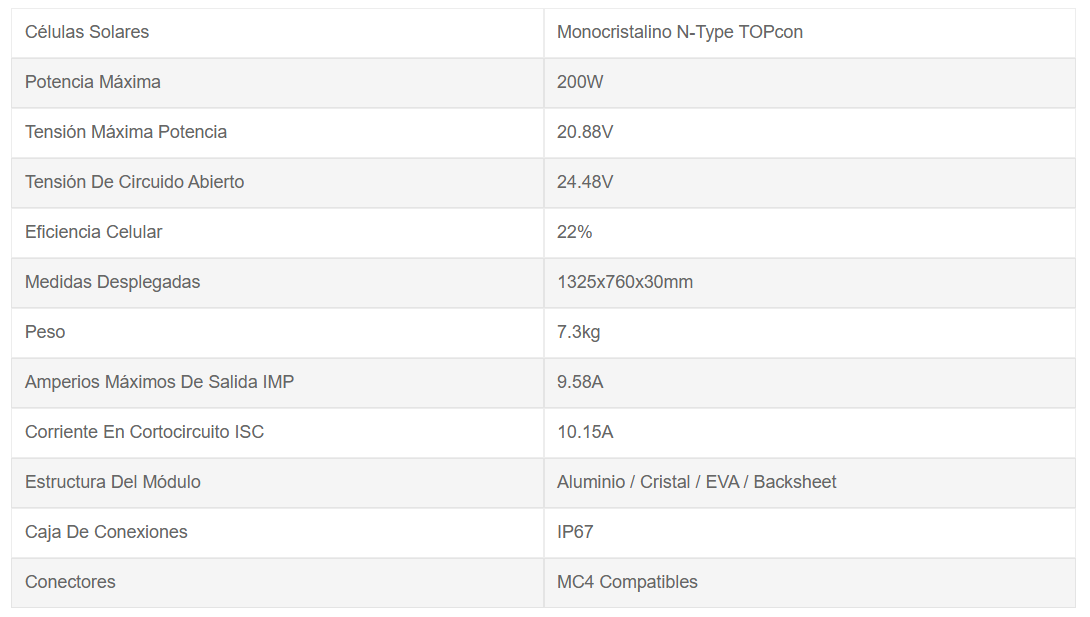
\includegraphics[width=0.7\textwidth]{images/2-hardware/Panel Solar/Caracteristicas.png}
        \caption{Prestaciones \texttt{SOLARIMPUT PF200T}}
        \label{fig:4-1-1-PanelSolar}
    \end{figure}
\end{itemize}

Todas estas características se han obtenido de la hoja de características aportada por el fabricante.\cite{semperesolutionsPanelSolarMonocristalino}

Por otra parte, para garantizar la eficiencia y seguridad del sistema, hemos decidido incorporar el regulador de carga solar \texttt{LandStar LS1524}. Este componente aporta un papel importante en la regulación del flujo de energía entre el panel solar y las baterías, previniendo sobredescargas, sobrecargas y garantizando más tiempo de vida útil al sistema.

De forma análoga al desarrollo realizado con el panel solar, a continuación se van a discutir las diferentes características de este regulador de carga solar.

\begin{itemize}
    \item \textbf{Compatibilidad con el sistema de carga}: El regulador de carga \texttt{LandStar LS1524} es compatible con sistemas de $12 V$ y $24 V$ lo que lo hace compatible con el panel solar seleccionado, el cual tiene una $V_{MP}$ de $20.88 V$. Además, tiene la capacidad de manejar corrientes de hasta 15A, más que suficiente para los $9.58 A$ de $I_{MP}$ que aporta nuestro panel solar.

    \item \textbf{Características técnicas}:
    \begin{itemize}
        \item \textbf{Regulación}: Este controlador utiliza regulación PWM o Modulación por Ancho de Pulso. Este método asegura una carga eficiente y una menor pérdida de energía durante la transferencia, actuando como un interruptor entre el panel y el circuito, forzando al módulo fotovoltaico a trabajar a la tensión deseada sin ningún tipo de instalación extra.
        \item \textbf{Protección}: Este modelo incluye protección contra cortocircuitos, sobredescarga y sobrecarga, asegurando la seguridad del panel solar y del circuito de carga.
        \item \textbf{Indicadores}: Este regulador incorpora diferentes LEDs, aportando información visual sobre el estado de carga y posibles fallos, facilitando el monitoreo del sistema.
    \end{itemize}

    \item \textbf{Eficiencia y robustez}: El controlador está diseñado para funcionar de manera eficiente en condiciones ambientales adversas. Además, su carcasa resistente y su fiable diseño electrónico, nos aseguran un correcto funcionamiento en aplicaciones en exteriores.

    \item \textbf{Prestaciones del regulador}:
    \begin{figure}[H]
        \centering
        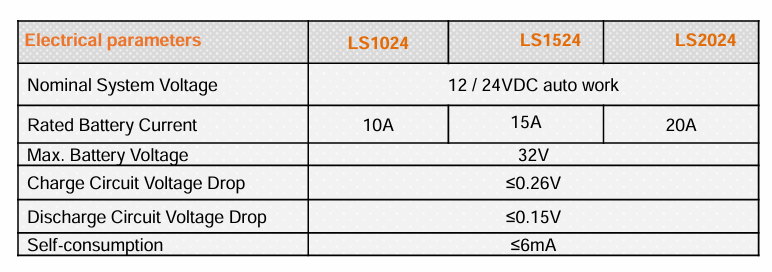
\includegraphics[width=0.6\textwidth]{images/2-hardware/Panel Solar/Regulador.png}
        \caption{Prestaciones \texttt{LandStar LS1524}}
        \label{fig:4-1-2-Regulador}
    \end{figure}
\end{itemize}

Todas estas características se han obtenido de la hoja de características aportada por el fabricante. \cite{epsolarLandStarSeriesSolar}

En conclusión, la combinación del panel solar \texttt{SOLARIMPUT PF200T} y el regulador de carga solar \texttt{LandStar LS1524}, constituyen una solución eficiente y fiable para los requisitos de nuestro sistema de carga de baterías. Por una parte, el panel solar ofrece las características técnicas necesarias para aportar la energía requerida por el sistema, mientras que el regulador de carga solar ofrece una correcta gestión de dicha energía y aporta una serie de protecciones que hacen al sistema más robusto y más seguro frente a posibles fallos. Ambos componentes garantizan una gran eficiencia, estabilidad y durabilidad al sistema, cumpliendo con los requisitos mínimos estimados y ofreciendo un gran equilibrio entre prestaciones y costes. Obtenido un flujo de corriente como el siguiente:

\begin{figure}[H]
    \centering
    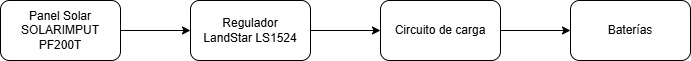
\includegraphics[width=0.7\textwidth]{images/2-hardware/Panel Solar/DiagramaBloquesPanel.jpg}
    \caption{Flujo de Corriente Panel Solar}
    \label{fig:4-1-2-FlujoCorrientePanel}
\end{figure}

